\chapter{Transport mode application to heavy-flavor evolution}
In this chapter, we shall start to focus on applying the LIDO transport model to the heavy-flavor section, and discuss in detail how a transport model fits into the complex dynamics that heavy flavor particles undergoes in the heavy-ion collision environment.

Heavy flavor is a charming probe for the medium created in heavy-ion collisions. 
Its large mass guarantees an negligible thermal production contribution at least for present LHC top beam energies for heavy-ion program (there are estimates that thermal contribution can play a row in future FCC collider).
Therefore, heavy flavors are almost always created in initial hard processes. 
By hard processes, it includes both the hardest few body collisions, as well as the associated high-virtuality parton evolution.
Their dilute population also suppresses the chances that they annihilates against their anti-particles during the medium evolution.
As a result, heavy flavors are created at relatively early stages of the heavy-ion collision and experienced the entire medium evolution and encodes valuable information about the medium.
On the theory side heavy flavor has a rich variety of physics interests. 
At high $p_T$, the evolution of heavy flavor particles merges into the context of jet dynamics and jet energy loss study; at intermediate $p_T$ the mass hierarchy predicted for the medium modifications;
and low $p_T$, heavy flavor is one of the key messengers for the thermalization processes inside QGP due to its long relaxation time compared to light partons.
On the experimental side, their unique flavors, masses, and decay modes also give us the chance to reconstruct heavy flavor (heavy meson / baryon) observables directly.

There are two types of heavy quarks that are most relevant for nowadays hard-probes study, the charm quark with mass $1.3$ GeV, and the bottom quark with mass $4.2$ GeV.
The reason top quark ($173$ GeV) is out of our discussion is due to its extremely short life time ($\sim 5\times 10^{-25} \approx 0.15$  fm/$c$ in the rest frame) so it barely interacts with the QGP before it decays predominantly into bottom quarks.
Even though there has also been proposal for taking advantage of this short time scale to probe the temporal structure of the QGP in its early stages, we shall focus on the charm and bottom flavor in this thesis.

To build a comprehensive simulation framework for the fate of heavy quarks in relativistic heavy-ion collisions requires a multi-component and multi-stage modeling.
Here we summarize this simulation framework in the following flow chart as a guide line for this section, figure \ref{fig:flowchart}.

\begin{figure}
\centering
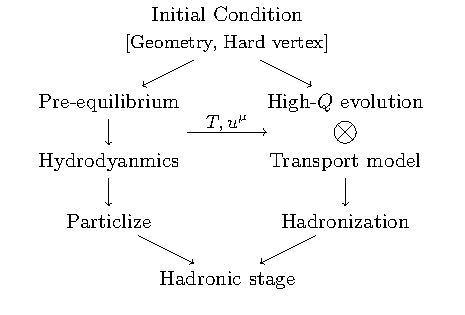
\includegraphics[width=.8\textwidth]{flowchart.pdf}
\caption{hh}
\label{fig:flowchart}
\end{figure}

In the previous two chapters, we have introduced the left branch of this flow chart, which is a relativistic viscous hydrodynamics based simulation for the bulk medium evolution.
The right branch is a model for the hard parton (heavy flavor) evolution.
The heavy quarks are produced in hard processes.
The hard processes contains both the hard matrix-element as well as the virtuality evolution of the parton (the DGLAP evolution or termed vacuum-like evolution).
One complication in the presence of medium, one complication is that vacuum-like evolution starts to occupied the same space-time of the medium induced processes at low-virtuality.
And should one interfaces the two calculations is still an interesting topic under debate.
One of the many obstacles is that multiple emissions / branchings are treated very differently in the two calculations.
For the vacuum-like evolution, the evolution variable is the virtuality scale with the space-time information integrated out, while the transport model evolves the systems in time, with virtuality integrated out below a certain scale.
There are many recent progress in both theory developments and newly design event-generators to solve this problem.
In this chapter, we shall focus on one possible solution to interface the two in section 1.
The in medium propagation of parton requires the medium properties as input. 
To zeros order of approximation, we specify the medium with its flow velocity and the equilibrium temperature, although the viscous hydro provides far more off-equilibrium information. 
This is discussed in section 2.
The heavy flavor hadronization model is introduced in section 3, which is a previously developed model that interpolates high-$p_T$ fragmentation processes and low-$p_T$ in medium recombination production of heavy hadrons.
Finally, in section 4, we also briefly introduced how this simulation framework of open heavy flavor can be coupled to the quarkonium evolution, but for more details, please refers to the thesis work [].

\section{Initial production of heavy flavor}
The initial hard processes are computed using perturbative QCD based or related Monte-Carlo event generator.
The general set up for such a computation in proton-proton collision is the factorization theorem \ref{fig:factorization}.
Where the perturbative QCD calculation provides the physics at short distance (a hard scale $Q^2$): the partonic matrix-elements $\hat{\sigma}_{ij\rightarrow kl}$.
The partonic configuration inside the proton characterized by the parton-distribution function (PDF) and the hadronization of the final state parton into hadrons are non-perturbative inputs.
Although these non-perturbative objects general cannot be computed from first principal and has to be extracted from measurements, their scale evolution in $Q^2$ can be described in perturbative QCD, knowns as the DGLAP evolution equations.
This scale dependence comes from that the exclusive process  $i+j \rightarrow k+l$ described by the fixed order matrix-elements is always modified by the parton branching and virtual correction that is of order $\alpha_s \ln Q^2/\mu^2$.
These corrections takes into account the fact that the initial high-virtuality parton $i$ (or $j$) may also come from a splitting processes of low virtuality parton $i'$ (or $j'$) from the proton, including virtually correction. 
Similarly, the final state high virtuality parton $k$ (or $l$) may also splits into a low virtuality parton $k'$ (or $l'$) before it becomes a hadron, including virtual correction.
The same argument also applies to partons $i', j', k', l'$. 
Eventually, one gets a series of contribution where although each term contains an additional power of $\alpha_s$, but is magnified by $\ln Q^2/\mu^2$ if there is a large gap between the hard scale $Q^2$ and the PDF scale $\mu^2$ at which it is measured.
The DGLAP evolution equations resum these logarithmic contributions systematically to increase the predictive power of the perturbative calculation of the inclusive cross-section.
Moreover, a useful parton-shower picture can be built from the process and with a probabilistic interpretation and Monte Carlo technique, one can mimic the exclusive final states from these sequences of parton branching processes.

In our studies, we have tried to use both inclusive cross-section program as well as Monte-Carlo event generator to initialize the heavy quark production.
Next we will explain their merits and draw backs for our purposes.

\paragraph{Initialize from inclusive cross-section program}
We use FONLL (Fixed Order Next to Leading Log) to generate the inclusive production cross-section of heavy flavor at partonic level.
The FONLL program is a combination of the fixed order (NLO) massive matrix-elements and a massless resummation program.
It predicts the single inclusive differential cross-section $d^2\sigma/dydp_T$. 
Then, one can sample the initial heavy quark's momentum from this differential cross-section.
The advantages are
\begin{itemize}
\item[1.] Sampling / weighting the inclusive cross-section is fast.
\item[2.] Provide interface to nuclear PDFs.
\item[3.] First principal approach for proton-proton collision.
\end{itemize} 
However, there are also disadvantages, 
\begin{itemize}
\item[1.] It only predicts single particle distribution and one cannot initialize the correlation of the $Q-\bar{Q}$ pair. This is not a problem for open heavy flavor observables, but would be a problem for quarkonium study.
\item[2.] The space-time picture of the production process is lost. One do not know whether the virtuality evolution takes a finite amount of time. So we have to assume charms quarks are produced at proper time $t=0^{+}$, which is always before the in-medium transport. But later we will see that from event generator simulations, the evolution can take a finite amount of time, overlapping with the QGP evolution.
\item[3.] Lacking the exclusive final state. Again, it is not a problem for open-heavy flavor study. But to describe full jets, one really needs an exclusive partonic final state of the virtuality evolution to initilize the partonic transport model.
\end{itemize}

\paragraph{Initialize from Monte-Carlo event generator.}
\begin{figure}
\centering
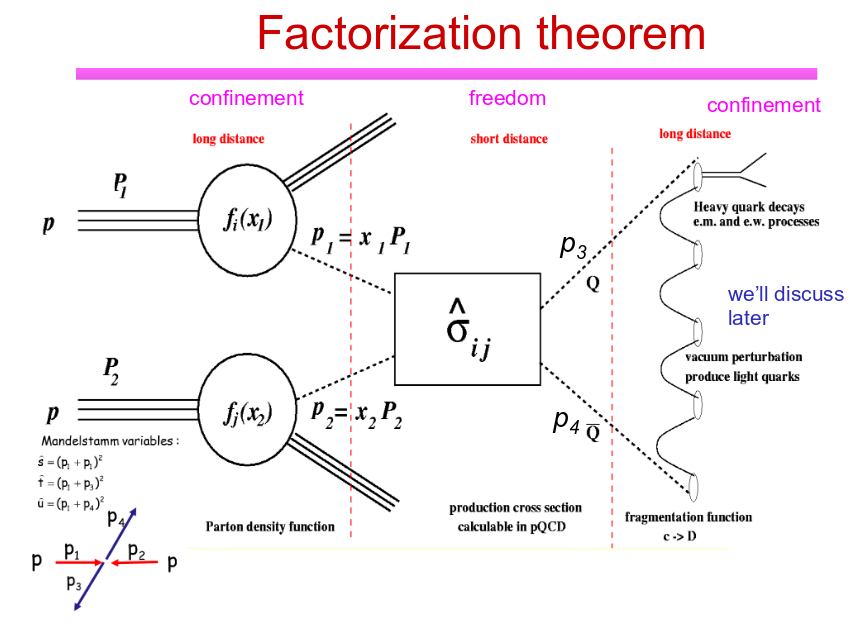
\includegraphics[width=\textwidth]{factorization.png}
\caption{
%https://indico.cern.ch/event/680421/contributions/3096162/attachments/1697092/2731944/J.Huston_Introduction_to_QCD_from_an_LHC_perspective-02.pdf
}
\label{fig:factorization}
\end{figure}

Another approach to generate initial hard process is to use high energy Monte-Carlo event generator, such as Pythia [].
Pythia implements the leading order (LO) matrix-elements for hard QCD processes, including LO production of heavy flavor particles,
$g+g\rightarrow Q+\bar{Q}$ and $q+\bar{q}\rightarrow Q+\bar{Q}$.
A parton shower will be generated based on the hard processes.
In fact, in high energy collisions, the LO production of heavy flavor is only a fraction of the total heavy flavor cross-section, the rest of them are created in the parton showers from the so-called gluon splitting and flavor creation processes.
The former corresponds to a situation where the heavy flavor pair comes from a final state gluon splitting; and the latter produces the pair in initial state gluon splitting and is put-on shell by the hard scattering.
These contributions also mimic certain pair correlations with non back-to-back angular correlations.

The disadvantage is of course the event generator is not a first principal computation of the heavy flavor production.
However, there are many benefits of having an exclusive final state.
\begin{itemize}
\item Although the parton shower is evolved as a function of virtuality $Q^2$. A qualitative space-time picture can be built by measuring the formation time of each branching by $2x(1-x)E/k_\perp^2$. In this way, we will see that the vacuum radiation off a heavy quark can last for a long time.
\item With the space-time picture, it is easier to analyze what kind of vacuum branchings should be modified in the presence of a medium.
\item Can be used to initialize the full transport model to study jets. 
\end{itemize}

\paragraph{Heavy flavor production baseline} In the course of our study, we used both the FONLL program and the Pythia event generator to initialize the momentum space. 
It is important to check that first whether they predict similar heavy flavor production in nuclear collisions and proton-proton collisions, and second if they provide good descriptions of the experimental measurement in proton-proton collisions.
In the upper plot of figure \ref{fig:pythia-fonll}, we compare the $p_T$ differential cross-section of $p+p\rightarrow c$ from FONLL calculations (lines) and from Pythia simulations (symbols), and for Pb+Pb collision (red) and p+p collision (blue) at the LHC energy $\sqrt{s}=5.02$ TeV.
For p+p system, we use the CT10 parton distribution function and for Pb+Pb system, the nuclear modification to the parton distribution is using the EPS09 parametrizaiton.

We note that the absolute value of the cross-sections are different.
Fortunately, the observables that we are interested in nuclear collisions are always ratios such as the nuclear modification factor $R_{AA}$, and the momentum-space anisotropy of heavy meson $v_n$ which is dimensional less. 
Therefore the shape of the spectra is the key feature we would like to compare between the two calculation and we have rescaled the FONLL curve.
We see that their shapes are very similar.
When calculation $R_{AA}$, we are dividing the cross-section from nuclear collision to that of the proton-proton collision.
To see how much the modulation in $R_{AA}$ is contributed by the nuclear PDF effects, we take the ratio between the AA and pp results in the upper plots to get an ``$R_{AA}$" for the nuclear PDF effects in the bottom plots.
We can see that FONLL and Pythia simulation predicts consistent modulation: the initial production AA spectra of charm quark at low-$p_T$ is suppressed compared to the pp spectra, due to the shadowing effect of the small-$x$ gluon. 
At higher $p_T$, the ratio increase and slightly shoots over  unity, this is because the there is an anti-shadowing region of the gluon at larger-$x$.

\begin{figure}
\centering
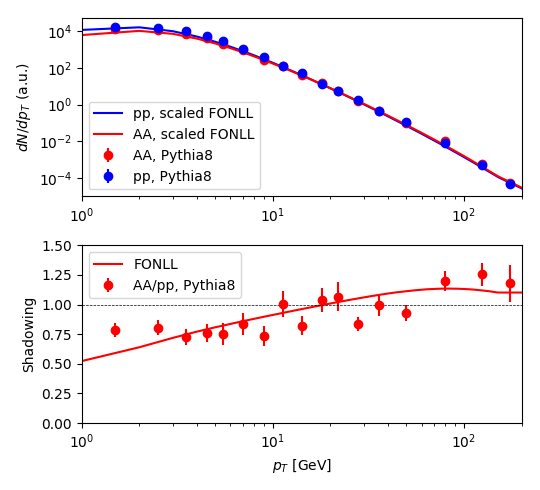
\includegraphics[width=.8\textwidth]{pythia-vs-fonll.png}
\caption{}
\label{fig:pythia-fonll}
\end{figure}

\section{Interfacing vacuum shower with in-medium transport}

\begin{figure}
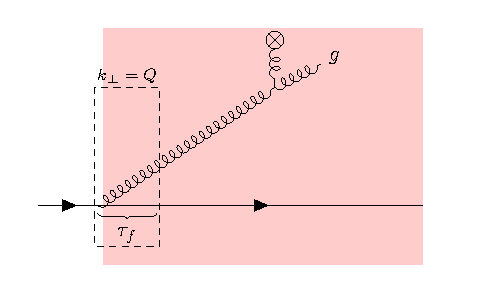
\includegraphics[width=.35\textwidth]{largeQ.pdf}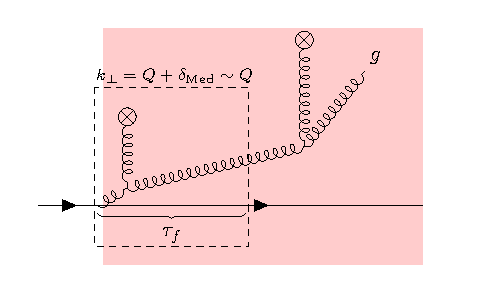
\includegraphics[width=.35\textwidth]{mediumQ.pdf}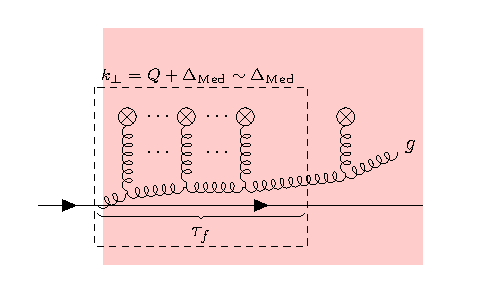
\includegraphics[width=.35\textwidth]{smallQ.pdf}
\caption{}
\label{fig:vac-med-interface}
\end{figure}
Interfacing the vacuum shower that evolves with virtuality and the transport equation that evolves with time is a difficult task. 
We shall provide a reasoning for the prescription we use following some of the recent developments [].
Start by considering a splitting of a hard parton which is created at the boundary of a brick medium.
This splitting has a formation time depending on its transverse momentum (or virtuality) $\tau_f \sim 2x(1-x)E/k_\perp^2$.
It is very likely that the radiated gluon (or the quark) interacts with a scattering center in the medium, denoted by the crossed circle.
If the virtuality of the splitting is very large, then the formation time is small.
The argument is that scatterings at time $t$ that is well separated from the formation time $\tau_f \ll t$ are independently from the initial vacuum-like splitting process; while scatterings within $\tau_f$ can change the branching probability.
So, we determine whether the vacuum branching should be modified in medium by the number of scatterings before $\tau_f$.

\begin{itemize}
\item For a branching with large virtuality (left of figure \ref{fig:vac-med-interface}) that $N = \tau_f/\lambda \ll 1$ (translates into $k_\perp^2 \gg \alpha_s  \omega T$). 
There chance for the medium interaction to modify the vacuum branching is negligible.
\item Hold the energy of the radiaion, while decrease its transverse momentum (middle of figure \ref{fig:vac-med-interface}) so that $N = \tau_f/\lambda \lesssim 1$ ($k_\perp^2 \gtrsim \alpha_s  \omega T$). 
Now, there is order one scatterings with the medium. 
The transverse momentum of the gluon is modified a little but still dominated by the initial virtuality.
The probability for the branching should also be modified.
For example, a higher twist expansion in terms of $1/k_\perp^2$ takes into account the effect of one interaction with the medium.
\item Further decreasing the initial virtuality of the branching (right of figure \ref{fig:vac-med-interface}) until $N = \tau_f/\lambda \gg 1$.
Now the final transverse momentum has to be determined self-consistently to be $k_\perp^2 \sim \sqrt{\hat{q}\omega} \sim \alpha_s\sqrt{\omega T^3}$. 
When this happens, the initial virtuality of the splitting is completely dominated by the medium effects (a medium scale at $\sqrt{\hat{q}\omega}$). 
And the branching probability should be replaced by a medium-induced calculation.
\end{itemize}
Summarizing the two extreme regions:
Vacuum branchings with $k_\perp^2 \gg \alpha_s \omega T$ is not modified, while branchings with $k_\perp^2 \sim \sqrt{\hat{q}\omega}$ should be treated as medium-induced process instead of vacuum radiation.
It is therefore natural to use $k_\perp^2$ and the fraction of $k_\perp^2$ that is contributed by the medium broadening $\Delta k_\perp^2$ to separate the medium-induced radiation and the vacuum-like radiation.
Since medium induced radiations treated by the transport equation always have $k_\perp^2 = \Delta k_\perp^2$,  our interfacing prescription is then to simply cut-out the vacuum branchings generated by Pythia in the region $k_\perp^2 <  \Delta k_\perp^2$ (this is also known as the vetoed region in the literature).

\begin{table}[h]
\centering
\caption{Treating Pythia branchings inside the medium}
\begin{tabular}{ccc}
\hline
\multirow{2}{*}{Formed inside medium} & $k_\perp^2 > C \Delta k_\perp^2$ & Unmodified\\
 & $k_\perp^2 < C \Delta k_\perp^2$ & Removed\\
Formed outside medium & Unmodified & \\
\hline
\end{tabular}
\label{tab:med-vac}
\end{table}

Since we are interested in heavy quarks, here we only concern the modification of the vacuum radiation off a heavy quark.
First, in the generated Pythia event, one searches for heavy flavor in the partonic final states and find all the gluons from its final state radiation (FSR).
Meanwhile, we add these gluons four momentum back to the heavy quark to define its four momentum at the original production vertex.
Using these information, we will ``redo'' the branching of this gluons along with the in-medium evolution in real time.
But this time, these gluons will not be separated from the heavy quark until it expires its formation time ($t-t_0>\tau_f$), meanwhile, elastic broadening is allowed.
When $t-t_0>\tau_f$, we have the information of the initial $k_\perp^2$ of the branching, and also the amount of elastic broadening $\Delta k_\perp^2$, and we apply the aforementioned perscription to decide whether  this branching is performed unmodified ($k_\perp^2>C\Delta k_\perp^2$) or ``removed'' ($k_\perp^2<C\Delta k_\perp^2$, as these branchings has already be treated by the transport equation).

In figure \ref{fig:lund}, we show the phase space occupied by the vacuum branching without medium (left) and the phase space occupied by the modified vacuum (blue color map) and the medium induced radiation (red contour) from our simulation framework.
It is presented on the lund diagram, where the vertical axis is $ln(1/x)$ ($ln(E/\omega)$), while the horizontal axis is $ln(1/\theta^2)$ ($\ln(\omega^2/k_\perp^2)$).
This arrangement is inspired by the character structure of the QCD splitting in the soft limit,
\begin{eqnarray}
dP \sim \frac{\alpha_s C_R}{\pi} \frac{dx}{x}\frac{d\theta^2}{\theta^2}
\end{eqnarray}
so that the distribution of the vacuum splitting on the lund diagram is mostly flat apart from running coupling effect.
On the left, we see that without the medium effect, the vacuum radiations fills the region below the lines $\tau_f < L_{med}$ and the non-perturbative bounds $k_\perp > 0.4$ GeV. 
Inside the medium, the medium-induced radiations distributed around the line $\theta^4\omega^3 = 2\hat{q}$ as expected, though the fluctuation is large.
The vacuum radiation in the phase-space region overlapped with the medium induced radiation is reduced, while the vacuum radiation with very short formation time (close to the origin) is unmodified.

\begin{figure}
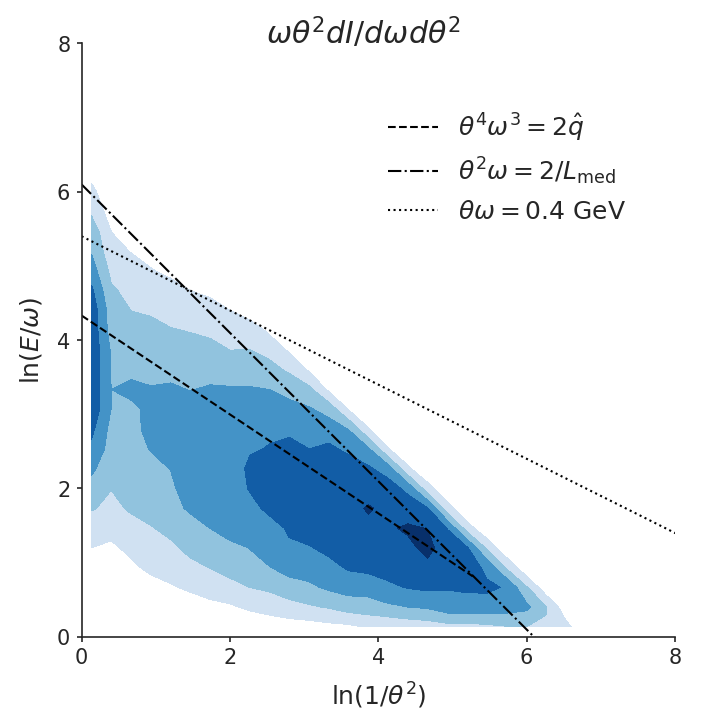
\includegraphics[width=.5\textwidth]{lund-vac.png}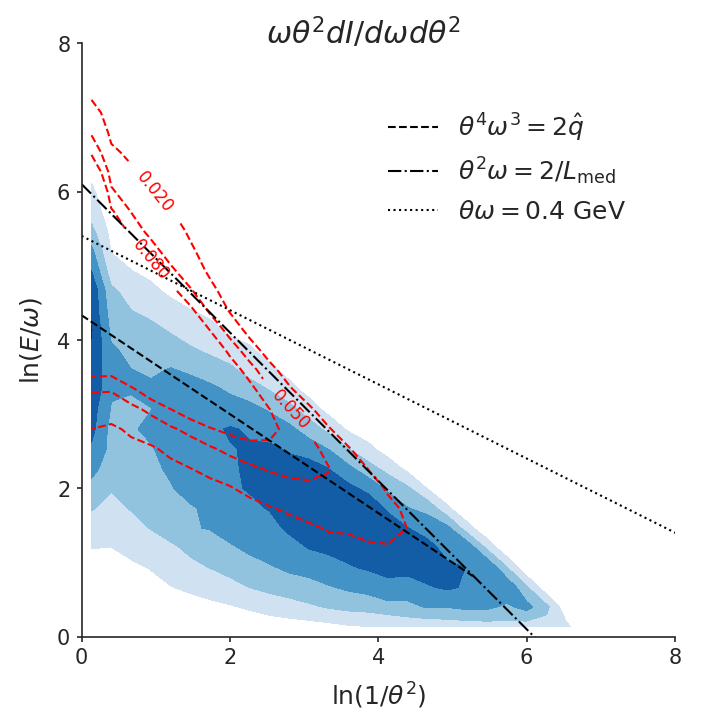
\includegraphics[width=.5\textwidth]{lund-med.png}
\caption{}
\label{fig:lund}
\end{figure}

To conclude this section, in order to interface the transport equation of medium-induced processes and the virtuality evolution of the vacuum radiation off a heavy quark, we redo the vacuum radiation of heavy quarks generated by Pythia along with the transport equations in time.
When the vacuum radiation forms at $t=\tau_f$, it is unmodified if the initial virtuality is greater than the acquired in-medium momentum broadening, otherwise it is removed.
On the Lund diagram, one can see that such the simulated medium-induced branchings and the vacuum branchings occupy different region of phase-space (with large fluctuation).
This procedure is, of course, only viable if we initialize the simulation with parton shower event generator.
We are not able to do such a ``subtraction" using heavy quark spectra calculated by FONLL.
 


\section{Coupling transport dynamics to an evolving medium}
The coupling between hydrodynamics and hard parton transport often require a switching of different reference frames, as the rest frame of the medium is also a function of space-time.
\paragraph{For diffusion dynamics} The diffusion equations is often written in the rest frame of the medium.
Therefore, one usually boost into the medium rest frame to update the momentum of the particle ($p_{M}^\mu$).
The transformation of the momentum is straight forward,
\begin{eqnarray}
p_{M}^\mu = L^\mu_\nu(\mathbf{v}_{M}) p_{L}^\nu
\end{eqnarray}
where $\mathbf{v}_{M}$ is the velocity of the fluid cell relative to the lab frame.
One needs to be careful with the time step in the fluid rest frame $\Delta t_{M}$, as it is not the same as the time step in the lab frame $\Delta t_{L}$.
Consider the world line the particle travels within $\Delta t_{L}$ of the lab frame and boost it into the medium frame
\begin{eqnarray}
\Delta x_{L}^\mu = \frac{p_{L}^\mu}{E_L} \Delta t_{L} \xrightarrow{\textrm{boost}} \Delta x_{M}^\mu = \frac{L^\mu_\nu(\mathbf{v}_{M}) p_{L}^\nu}{E_L} \Delta t_L = \frac{p_{M}^\mu}{E_L} \Delta t_L
\end{eqnarray}
Now compare the time-component of the equation, one get the time step in the medium frame is related to the lab frame step by the ratio between the energy of the particle in the two reference frames,
\begin{eqnarray}
\Delta t_M = \frac{E_M}{E_L} \Delta t_L
\end{eqnarray}
Once the momentum is updated in the medium frame to become $p'_M$, it is boosted back to the lab frame,
\begin{eqnarray}
x'^{\mu} &=& x^{\mu} + \frac{p_{L}^\mu}{E_L} \Delta t_{L} \\
p_{L}^{'\mu} &=& L^\mu_\nu(-\mathbf{v}_{M}) p_{M}^{'\nu}
\end{eqnarray}
where we have chosen to update position before the update of the momentum.

The choice of $\Delta t_L$ is also tricky. 
A uniform time step for all the particles in the medium sounds like the most straightforward solution, but it is not the optimal choice.
This is because the relativistic hydrodynamics for heavy-ion collision is often solved in the $(\tau,x,y,\eta_s)$ coordinates, and the hydrodynamic field is propagated from one constant proper time $\tau = \sqrt{t^2 - z^2}$ to the next.
There are two consequences if we choose the $\Delta t_L$ for all particles:
\begin{itemize}
\item The particles will be lying on different proper time $\tau$ at a constant $t$, and will requires the program to load the entire hydro solution into the memory, which can be a problem if one uses a 3+1D hydro simulation.
\item The medium-rest-frame time step for particles at large space-time rapidity would be too small. 
\end{itemize}
For these (mainly practical) reasons, we choose to propagate particles with a constant $\Delta \tau$ step. 
Then, each particle has its own clock depending on its spatial points and momentum,
\begin{eqnarray}
\Delta \tau = \sqrt{(t+\Delta t_L)^2 - (z+v_z \Delta t_L)^2} - \sqrt{t^2 - z^2}
\end{eqnarray}
which solves to be (keeping the positive solution),
\begin{eqnarray}
\Delta t_L(p, x) = \frac{-(t-z v_z) + \sqrt{(t-z v_z)^2 - (1-v_z^2)(\Delta \tau^2 + 2\sqrt{t^2 - z^2}\Delta \tau )}}{2(1-v_z^2)}
\label{eq:dt-transformation}
\end{eqnarray}
And then each particle uses this adaptive time step in the lap frame to propagate to the next constant proper-time hyper-surface.

\paragraph{For matrix-element scattering} The situation for coupling the matrix-element scatterings is more complicated as a third reference frame appears: the center-of-mass frame of the two-body and three-body collisions.
This is because while sampling the initial state of scattering is straightforward in the medium rest frame, the final state sampling is mostly easy done in the center-of-mass frame.
The work-flow proceed as,
\begin{itemize}
\item For each hard parton, determine $\Delta t_L$ with equation \ref{eq:dt-transformation}.
\item Boost the particle to the medium rest-frame and sample the scattering rate $\Delta t_M R$ channel, and then sample the medium parton(s) that forms the scattering initial state with the hard parton.
\item In the CoM frame of the initial state, sample the final state particles.
\item Boost back the final state particles to the medium rest frame.
\item Boost back to the lab frame.
\end{itemize}

\section{Heavy-flavor hadronization and hadronic stage}
The hadronization model for the heavy flavor is the simulation is implemented by [].
It is a sudden hadronization of heavy quarks into heavy hadrons at a constant medium temperature hypersurface, and combines the fragmentation of heavy quark at high momentum and the recombination with medium partons into hadrons at low momentum.

\paragraph{The ``sudden" approximation} the hadronization is treated to be instantaneous on a isothermal hypersurface.
This approximation certainly has its drawbacks.
First, hadronization is a long distance process. 
In the rest frame of the heavy flavor, it takes time scale $1/\Lambda_{QCD}$. 
With a large boost factor $E/M_{\textrm{hadron}}\sim E/M_{\textrm{heavy quark}}$, the formation time of the heavy hadron can be comparable to the macroscopic length scale.
For example, for a moderate $E=10$ GeV charm quark $M=1.3$ GeV, this time is estimated to be $8$ fm/c, which is certainly not a sudden process considering the hydrodynamic stage only last for $O(10)$ fm/$c$.
Second, an instantaneous recombination process breaks energy conservation and detailed balance, as will be shown below.
To solve these problems, one really needs a dynamical modeling of the hadronization physics in the future,
which is already a hard problem even in the vacuum.


\paragraph{Recombination}
The recombination model was introduced in []. 
The basic idea is that the probabilities for a heavy quark to recombine with medium parton(s) into heavy mesons and baryons are calculated as the wave-function overlap of the initial state quark wave-function and final state hadron wave-function, integrated over the thermal distribution of the medium parton,
\begin{eqnarray}
\frac{dP_{p_Q \rightarrow p_M}}{dp_M^3} &=& \int dp^3_{\bar{q}} n_{\bar{q}} f^W_{M}(\vec{p}_Q, p)\delta^{(3)}(\vec{p}_M-\vec{p_Q}-\vec{p}) \\
\frac{dP_{p_Q \rightarrow p_B}}{dp_B^3} &=& \int dp^3_{q}dp'^3_{q'} n_{q} n_{q'} f^W_{B}(\vec{p}_Q, p, p')\delta^{(3)}(\vec{p}_B-\vec{p_Q}-\vec{p}-\vec{p}') 
\end{eqnarray}
On the left are the differential probability for a heavy quark with momentum $p_Q$ to hadronize into a heavy meson or a heavy baryon through recombination.
They are equal to Wigner function overlap $f^W$ for meson and baryon integrated over light quark / anti-quark distribution function, subject to momentum conservation.
Here, it is evident that a energy conservation is not imposed in this instantaneous $2\rightarrow 1$ coalescence approach.
The quark / anti-quark distribution function is the Fermi-Dirac one, neglecting the chemical potential, 
\begin{eqnarray}
n = \frac{g_q V}{e^{\beta p\cdot u} + 1}
\end{eqnarray}
with $u$ the fluid velocity and the $p$ the four momentum of the light quark / anti-quark.
$g$ is the degeneracy of the quark, and $V$ is a test volume that will eventually be canceled by the normalization factor in the the Wigner function.
As a remark, we have assumed in the transport model that the thermal partons are massless, since the thermal mass contribute one extra power of $g$ and is not included in the leading order computation.
However, for the recombination near the critical temperature, non-perturbative constituent masses are assigned to light quarks, $m_u = m_d = 300$ MeV and $m_s = 475$ MeV.
Modeling the meson wave-function $\phi_M$ with a Gaussian form and the meson Wigner function can be computed as,
\begin{eqnarray}
\phi_M(\vec{r}) &=& \left(\frac{1}{\pi \sigma^2}\right)^{3/4} e^{-\frac{r^2}{2\sigma^2}}\\
f_M^{W}(\vec{r}, q^2) &=& g_M N \int d^3 \vec{a} e^{-i\vec{q}\cdot \vec{a}} \phi_M(\vec{r}+\vec{a}/2) \phi_M^*(\vec{r}-\vec{a}/2) \\
f_M^{W}(q^2)  &=& \frac{g_M N}{V} (2\sqrt{\pi}\sigma)^3 e^{-\sigma^2 q^2}, \vec{q} = \frac{E_2\vec{p}_1 - E_1\vec{p}_2}{E_1+E_2}
\end{eqnarray} 
Where in the last step, a spatial averaged Wigner function within the test volume $V$ is defined.
And the transition probability is,
\begin{eqnarray}
\frac{dP_{p_Q \rightarrow p_M}}{dp_M^3} &=& N\int dp^3_{\bar{q}} \frac{g_q g_M}{e^{\beta p\cdot u} + 1} (2\sqrt{\pi}\sigma)^3 e^{-\sigma^2 q^2} \delta^{(3)}(\vec{p}_M-\vec{p_Q}-\vec{p})
\end{eqnarray}
One can see the cancellation of the test volume in the distribution function and the Wigner function.
The $\sigma$s are the key parameters, and is related to the reduced mass of the two body system $\mu = m_1 m_2/(m_1+m_2)$ and the frequencty of the  potential $\omega$ by $\sigma = 1/\sqrt{\mu \omega}$.
These frequency is estimated from the charge radius of different heavy mesons to be $0.106$ GeV for charmed hadron and $0.059$ GeV for the bottom mesons.

The same can be applied to heavy baryon recombination, with the three-body Wigner function in the Gaussian approximation as,
\begin{eqnarray}
f_B^W(q_1^2, q_2^2) = \frac{N g_B}{V^2} (2\sqrt{\pi\sigma_{1,2}\sigma_{12,3}})^6 e^{-q_{1,2}^2 \sigma_{1,2}^2 - q_{12,3}^2 \sigma_{12,3}^2}.
\end{eqnarray}
With the three body system analyzed as a two ``two-body system'' between the pair $p_1$ and $p_2$, and between the composite pair $p_3$ and $p_1+p_2$, so that
\begin{eqnarray}
\vec{q}_{1,2} &=& \frac{E_2 \vec{p}_1 -E_1\vec{p}_2}{E_1+E_2}\\
\vec{q}_{12,3} &=& \frac{E_3 (\vec{p}_1+\vec{p}_1) - (E_1+E_2)\vec{p}_3}{E_1+E_2 + E_3}\\
\sigma_{1,2}^{-1} &=& \sqrt{\omega \frac{m_1m_2}{m_1+m_2}}\\
\sigma_{12,3}^{-1} &=& \sqrt{\omega \frac{(m_1+m_2)m_3}{m_1+m_2+m_3}}
\end{eqnarray}

\paragraph{Fragmentation} At high momentum, heavy quark hadronize through the fragmentation mechanism that produces a heavy hadron that carries a certainty fraction of the origin quark energy $z = p_H/p_Q$.
The probability distribution of $z$ is known as the fragmentation function, and here the Peterson parametrization is used,
\begin{eqnarray}
f(z) \propto \frac{1}{z(1-\frac{1}{z} - \frac{\epsilon}{1-z})^2}
\end{eqnarray}
where $\epsilon$ is a parameter that dependences on the heavy quark mass.

To synthesis the competing mechanisms of fragmentation and recombination that dominates at high momentum and low momentum respectively, one first samples the recombination probability and determines whether the heavy quark coalesces with the medium partons. 
If not, its hadronization will be handled by the Pythia fragmentation routine with the Peterson fragmentation function.

\section{Coupling open-heavy flavor to quarkonium evolution}
